% !TEX root =/main.tex
\chapter{Introduction}
\section{Introduction to C}
\begin{snippet}{Code snippet 1.0}
	\begin{lstlisting}
		#include <stdio.h> // Tells the preprocessor to load a file

		int main() 			// The entrypoint of the program
		{						// Defines a block of code, everything created in it and not returned is only defined for the block
			printf("Hello world\n");	// A basic statement
			return 0;
		}
	\end{lstlisting}
\end{snippet}

For this course we will use Chalmers remote StuDat computers.

\section{Course introduction}

The course book is "Modern Operating Systems", by Tanenbaum and Bos.

Vincenso should work on his standup comedy.

\subsection{Why study OS?}

Provides services to system users. Studying it gives us an overview of how computers work on a lower level.

The operating system is both there to help the user actually use the computer, but also to protect the hardware from the main source of complications; the user. It makes sure that everything that needs to run on the computer is able to do so, and is given sufficient resources to perform its task.

\section{What is an Operating system}
An operating system is a program which provides a \textit{set of services} to system users (human users and computer programs). It also protects the user from the hardware and vice verse.

An operating system manages resources on the computer and makes sure that all system users get the necessary resources (if possible), such as cpu(s), memory to store data, i/o devices and so on.
It controls the execution of different programs, makes sure that an error in one doesn't cascade into others and makes sure different programs stay independent and cannot access each others' resources.

\begin{example}{Saving a file}
	When the user is saving a file, without an operating system, nothing else would be able to happen on the computer while waiting for that; with a good operating system, the hardware resources can be managed in such a way that other tasks can be performed while waiting for the file to be written.
\end{example}

\section{The event-driven (interrupt-drive) life of an OS}
\begin{figure}[H]
	\centering
	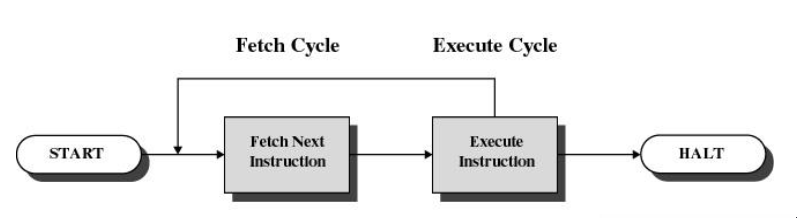
\includegraphics[width=0.4\textwidth]{images/fetch_cycle_simple.png}
	\label{fig:simple_fetch_cycle}
	\caption{A simple fetch cycle where only one thing happens}
\end{figure}
\begin{figure}[H]
	\centering
	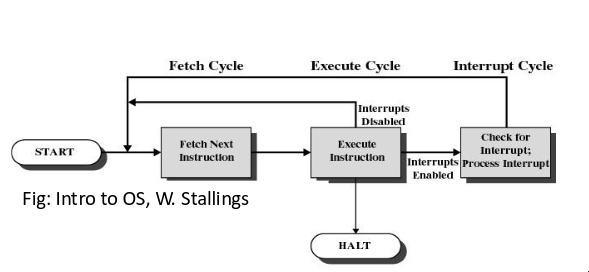
\includegraphics[width=0.4\textwidth]{images/fetch_cycle_advanced.png}
	\label{fig:advanced_fetch_cycle}
	\caption{A more advanced fetch cycle where things can happen in the background}
\end{figure}

\begin{minipage}{0.65\textwidth}
	By looking for interrupts between running the instructions we are able to handle events from different parts of the system. With this we can achieve what was talked about in the example above, where other programs execute while the saving of a file was happening.

	Scheduling is about choosing for how long a certain program can run before it needs to be interrupted for another program to be able to run. It is the operating system's job to choose for how long, and to choose the order the processes gets to run.
\end{minipage}
\begin{minipage}{0.3\textwidth}


	\begin{figure}[H]
		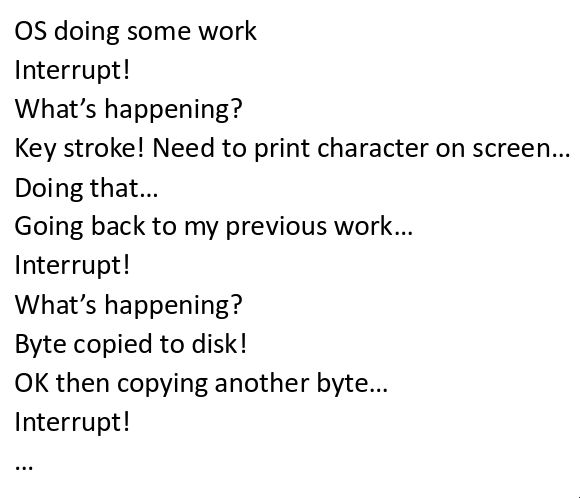
\includegraphics[width=1\textwidth]{images/os_event_cycle.png}
		\label{fig:os_event_cycle}
		\caption{An example of a basic event cycle.}
	\end{figure}
\end{minipage}

\section{System calls (overview)}
System calls are ways for user programs to \textit{''talk to''} the hardware. All actions a user wants to do which modifies the hardware requires a system calls, e.g. Creating files, sending data over internet, showing something on a screen; are created through system calls. All system calls are types of interrupts. When the CPU finds the interrupt, control is given to the operating system, which chooses how to do the thing the user wants to do (if possible and the user should be able to).

\section{Dual-Mode and Multimode Operation}
What happens if a user tries to bypass the operating system by directly modifying the hardware without using system calls? The hardware keeps track of what kind of program is running, when the operating system is running, a bit is set which allows it to run ''special functions'' that normal users cannot.

To make sure the user cannot set that bit for themselves, when the hardware first starts, it loads the operating system into memory; during this phase the hardware and operating system defines which operations are privileged, and what code to run when those actions are performed. When the user tries to do those privileged actions, for example modifying a file, the operating system starts running.
\section{Operating system services}
\section{System calls (continued) and APIs [Self reading]}
\section{System boot [Self reading]}
\section{Operating systems structures}